\documentclass[11pt,a4paper]{article}
\usepackage[utf8]{inputenc}
\usepackage[T1]{fontenc}
\usepackage[brazilian]{babel}
\usepackage{amsmath,amssymb,mathtools,booktabs,graphicx,float}
\usepackage[margin=2.2cm]{geometry}
\graphicspath{{resultados/}}

\title{Teoria da Informação -- Primeira Atividade em Grupo\\
       \large Relatório das Simulações}
\author{Gabriel Takeuchi (13671636) \and Gabriela Victor (11795381) \and Francisco Membrive (12553782) \and Octavio Carneiro (13831609) \and Fernando Lima (13672710) \and Pedro Bonifácio (14602244) \and Ulisses Cordeiro}
\date{}

\begin{document}
\maketitle

%======================================================================
\section{Tópico 1: Entropia, Informação Mútua e Teste de Independência}

\subsection{Modelo de diagnóstico, convergência e custo de codificação}
Definimos o modelo probabilístico do teste rápido de dengue com prevalência $p(D=1)=0{,}10$, taxa de falso positivo $p(T=1\mid D=0)=0{,}05$ e taxa de falso negativo $p(T=0\mid D=1)=0{,}20$. A partir de uma amostra simulada de $N=5\,000$ pacientes, construímos a tabela de contingência $2\times2$ e calculamos as entropias e a informação mútua pelas frequências relativas empíricas. A Tabela~\ref{tab:t1_p3} mostra que as estimativas ficaram bem próximas dos valores teóricos, preservando exatamente as identidades $H(D\mid T)=H(D,T)-H(T)$ e $I(D;T)=H(D)-H(D\mid T)\approx 0{,}214$ bits.

\begin{table}[htbp]
  \centering
  \caption{Comparação entre valores teóricos e estimados na amostra ($N=5\,000$).}
  \label{tab:t1_p3}
  \begin{tabular}{lrrr}
\toprule
Quantidade & Teórico & Estimado ($N=5000$) & Diferença \\
\midrule
$H(D)$ & 0.4690 & 0.4490 & -0.0200 \\
$H(T)$ & 0.5436 & 0.5077 & -0.0359 \\
$H(D,T)$ & 0.7989 & 0.7516 & -0.0474 \\
$H(D|T)$ & 0.2554 & 0.2438 & -0.0115 \\
$I(D;T)$ & 0.2136 & 0.2052 & -0.0084 \\
\bottomrule
\end{tabular}

\end{table}

Para analisar o comportamento do estimador em função do tamanho amostral, repetimos a simulação 500 vezes para $N\in\{20, 50, 100, 500, 2\,000, 10\,000\}$, tanto no modelo real quanto em um cenário com $D$ e $T$ independentes ($I=0$). Como ilustrado na Figura~\ref{fig:t1_p4}, o erro quadrático médio diminui conforme $N$ cresce, mas amostras pequenas sofrem com um viés positivo sistemático: para $N=20$, obtemos em média $\hat I\approx 0{,}248$ bits no modelo dependente e $\hat I\approx 0{,}039$ bits sob independência. Esse viés decorre da relação assintótica $2N\ln(2)\,\hat I \sim \chi^2_1$, cuja esperança implica $E[\hat I]\approx 1/(2N\ln 2)\approx 0{,}036$ bits para $N=20$.

\begin{figure}[htbp]
  \centering
  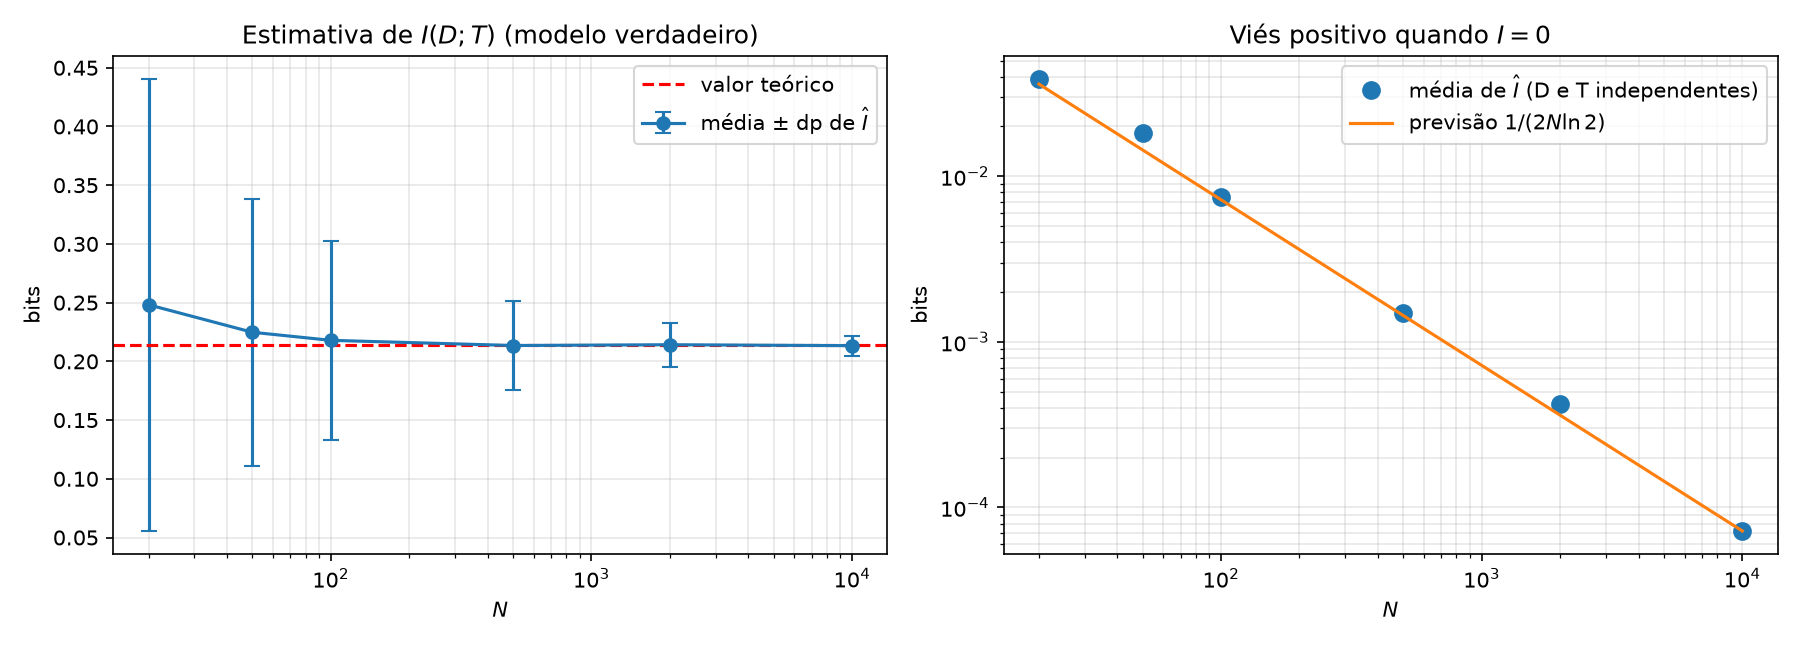
\includegraphics[width=0.92\textwidth]{fig_t1_passo4.png}
  \caption{Convergência de $\hat I(D;T)$ com o tamanho da amostra (esquerda) e viés positivo sob independência comparado à aproximação teórica $1/(2N\ln 2)$ (direita).}
  \label{fig:t1_p4}
\end{figure}

Avaliamos também o efeito de projetar a codificação assumindo uma distribuição incorreta $q(D=1)=0{,}30$. O custo teórico médio passa de $H(p)=0{,}4690$ para a entropia cruzada $H(p,q)=0{,}6368$ bits, resultando em um excesso igual à divergência de Kullback-Leibler $D(p\|q)=0{,}1678$ bits por paciente. Na amostra simulada, a diferença entre os comprimentos médios ideais ($-\log_2 q(d)$ versus $-\log_2 p(d)$) foi de $0{,}1799$ bits, ligeiramente acima do valor teórico devido à flutuação da frequência amostral de infectados ($9{,}4\%$). Além disso, verificamos a assimetria da divergência, uma vez que $D(q\|p)=0{,}2217 \neq D(p\|q)$.

\subsection{Dependência temporal e teste de independência}
Para incorporar a persistência temporal nos resultados de um mesmo paciente ao longo de $n=8$ dias, simulamos $200\,000$ históricos a partir de uma cadeia de Markov de dois estados com matriz de transição $P=\begin{psmallmatrix}0{,}9&0{,}1\\0{,}2&0{,}8\end{psmallmatrix}$, iniciada na distribuição estacionária $\pi=(2/3, 1/3)$. No primeiro dia, a incerteza é $H(T_1)\approx 0{,}918$ bits; a partir do segundo dia, a entropia condicional estabiliza em $\hat H(T_i\mid T_1,\dots,T_{i-1})\approx \hat H(T_i\mid T_{i-1})\approx 0{,}553$ bits, confirmando que dias anteriores a $i-1$ não trazem informação adicional dado o dia imediatamente anterior. Pela regra da cadeia, o histórico completo requer $H(T_1,\dots,T_8)\approx 4{,}78$ bits, contra $8H(T_1)\approx 7{,}34$ bits da transmissão independente dia a dia. A economia obtida é de $2{,}56$ bits por histórico de 8 dias, valor que coincide com $(n-1)I(T_i;T_{i-1})\approx 7\times 0{,}365$ bits.

Por fim, aplicamos o teste de independência baseado na estatística $G = 2N\ln(2)\,\hat I \sim \chi^2_1$ ($\alpha=5\%$). Na amostra principal, o teste rejeitou com folga a hipótese nula tanto para o par $(D,T)$ ($G=1422{,}2$, $p\ll 0{,}001$) quanto para dias consecutivos $(T_i,T_{i-1})$ ($G=1045{,}5$, $p\ll 0{,}001$), coincidindo exatamente com os resultados de \texttt{scipy.stats.chi2\_contingency} (com \texttt{correction=False}, já que a correção de Yates altera o valor em tabelas $2\times2$). Repetindo o teste 1\,000 vezes em três regimes (Tabela~\ref{tab:t1_p10}), vemos que sob dependência forte o poder é próximo de $100\%$ já para $N=100$, enquanto no cenário de dependência fraca ($I\approx 0{,}0026$) o poder sobe de $10{,}6\%$ ($N=100$) para $75{,}3\%$ ($N=2\,000$). Sob independência real, a taxa de rejeição fica próxima dos $5\%$ esperados para $N\ge 500$, mas sobe para $6{,}9\%$ em $N=100$, pois $96{,}2\%$ das tabelas geradas possuem células com contagem esperada menor que 5, comprometendo a aproximação qui-quadrado.

\begin{table}[htbp]
  \centering
  \caption{Taxa de rejeição de $H_0$ ($\alpha=5\%$) em 1\,000 repetições para diferentes cenários e tamanhos de amostra.}
  \label{tab:t1_p10}
  \begin{tabular}{lrrrr}
\toprule
Cenário & $I(D;T)$ & $N$ & Rejeições de $H_0$ & Tabelas c/ esperado $<5$ \\
\midrule
Forte & 0.2136 & 100 & 99.8\% & 100.0\% \\
Forte & 0.2136 & 500 & 100.0\% & 19.2\% \\
Forte & 0.2136 & 2000 & 100.0\% & 0.0\% \\
Fraca & 0.0026 & 100 & 10.6\% & 76.3\% \\
Fraca & 0.0026 & 500 & 27.0\% & 0.0\% \\
Fraca & 0.0026 & 2000 & 75.3\% & 0.0\% \\
Independente & $-8.65\times 10^{-17}$ & 100 & 6.9\% & 96.2\% \\
Independente & $-8.65\times 10^{-17}$ & 500 & 4.8\% & 0.0\% \\
Independente & $-8.65\times 10^{-17}$ & 2000 & 4.4\% & 0.0\% \\
\bottomrule
\end{tabular}

\end{table}

%======================================================================
\section{Tópico 2: Desigualdade de Processamento de Dados}

\subsection{Cadeia de canais ruidosos e pipeline de classificação}
Simulamos o envio de um bit uniforme $X$ através de $k=10$ canais binários simétricos (BSC) em série, propagando $N=200\,000$ mensagens independentes. Como a composição de $j$ canais BSC($p$) equivale a um único BSC com probabilidade de inversão $p_j = \frac{1-(1-2p)^j}{2}$, a informação mútua teórica no elo $j$ é $I(X;Y_j) = 1 - H_b(p_j)$. A Figura~\ref{fig:t2_p56} mostra que $\hat I(X;Y_j)$ cai monotonicamente a cada etapa: para $p=0{,}1$, parte de $0{,}529$ bits no primeiro elo e chega a $0{,}008$ bits no décimo; para ruídos mais altos ($p=0{,}2$ e $0{,}3$), a informação se dissipa já nos primeiros estágios. Também verificamos na amostra que $\hat I(X;Y_2\mid Y_1)\approx 0$, como esperado pela propriedade de Markov. Em testes auxiliares com amostras pequenas ($N=200$), observamos pequenas oscilações positivas na curva estimada entre um elo e o seguinte, que desaparecem ao aumentar $N$, confirmando tratar-se apenas de variância amostral do estimador.

\begin{figure}[htbp]
  \centering
  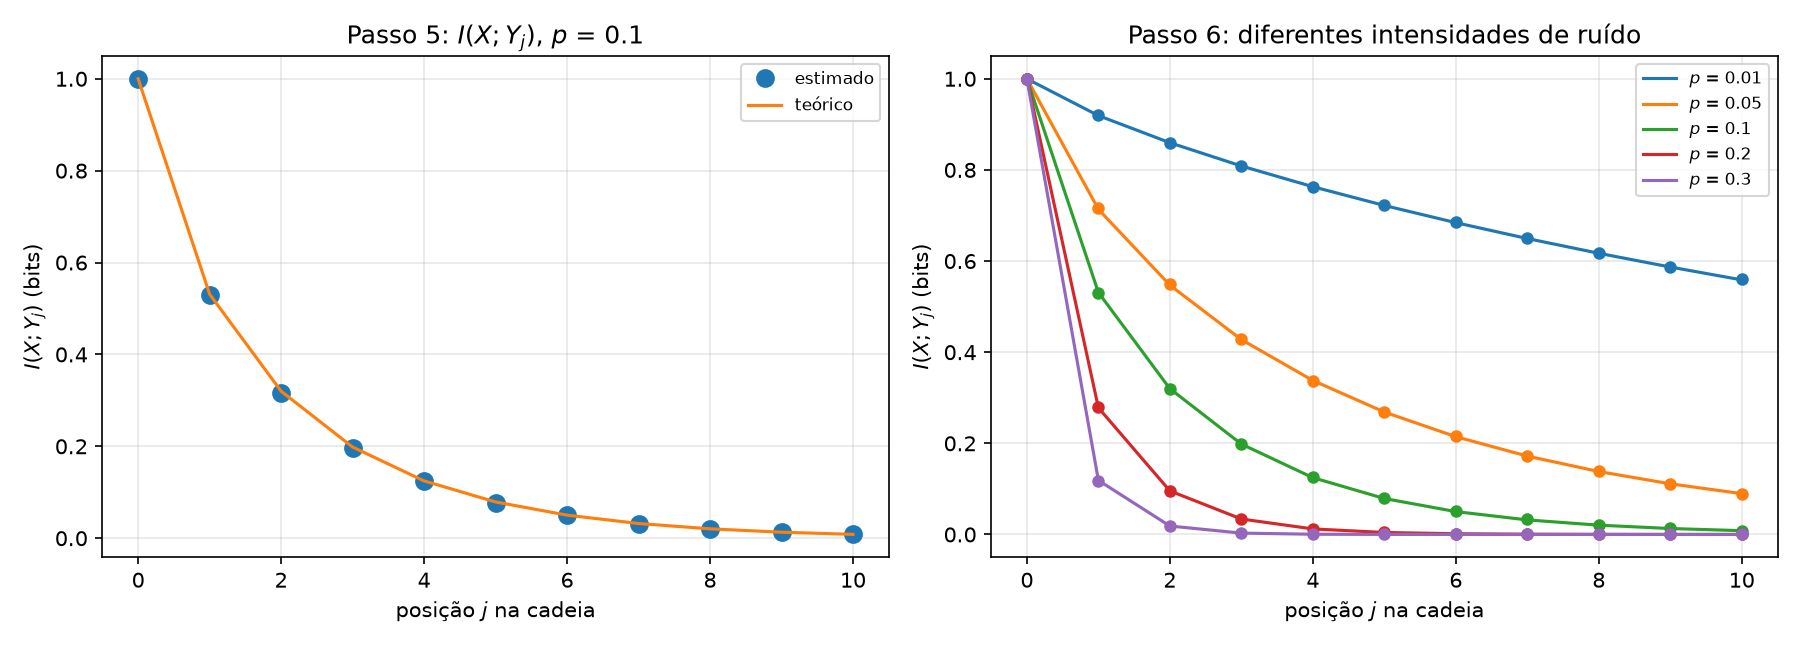
\includegraphics[width=0.92\textwidth]{fig_t2_passo5_6.png}
  \caption{Degradação da informação mútua $I(X;Y_j)$ ao longo dos 10 elos da cadeia para $p=0{,}1$ (esquerda) e comparação entre diferentes níveis de ruído (direita).}
  \label{fig:t2_p56}
\end{figure}

Em seguida, implementamos um pipeline em três etapas inspirado em aprendizado de máquina: o rótulo verdadeiro $X\in\{0,1\}$ gera uma ``imagem'' ruidosa $\mathbf Z\sim\mathcal N(\boldsymbol\mu_X,\mathbf I_{16})$ em $\mathbb R^{16}$ (com $\boldsymbol\mu_0=\mathbf 0$ e $\boldsymbol\mu_1=0{,}4\,\mathbf s$, sendo $\mathbf s\in\{-1,+1\}^{16}$), que é comprimida em um vetor de dimensão 4 tomando-se a média de blocos de 4 coordenadas e, por fim, classificada pela menor distância euclidiana às médias comprimidas. Para estimar a informação mútua nos estágios contínuos sem discretizar diretamente os espaços de 16 e 4 dimensões, projetamos os vetores na log-razão de verossimilhança (que é uma estatística suficiente unidimensional e, portanto, preserva $I(X;\mathbf Z)$) e discretizamos o resultado em 50 faixas de quantis. A Tabela~\ref{tab:t2_p8} confirma a desigualdade de processamento de dados ao longo do pipeline: a compressão reduz a informação de $0{,}353$ para $0{,}132$ bits (pois parte do sinal se cancela nas médias em bloco), e o classificador final retém $0{,}088$ bits (associado a um erro de classificação de $32{,}7\%$), sem conseguir recuperar o que foi perdido na etapa anterior.

\begin{table}[htbp]
  \centering
  \caption{Informação mútua entre o rótulo $X$ e cada estágio do pipeline de classificação.}
  \label{tab:t2_p8}
  \begin{tabular}{lrrr}
\toprule
Estágio & Dimensão & $\hat I(X;\cdot)$ & $I(X;\cdot)$ teórico \\
\midrule
Imagem completa & 16 & 0.3534 & 0.3527 \\
Representação comprimida & 4 & 0.1319 & 0.1314 \\
Predição final & 1 & 0.0881 & 0.0878 \\
Erro de classificação &  & 0.3271 & 0.3274 \\
\bottomrule
\end{tabular}

\end{table}

\subsection{Colapso de modelo em gerações sucessivas}
Para simular o fenômeno de colapso de modelo, consideramos uma distribuição original $p_{\text{real}}$ sobre $K=10$ categorias seguindo uma lei de Zipf ($H(p_{\text{real}})\approx 2{,}87$ bits). Na geração 0, sorteamos $n$ exemplos de $p_{\text{real}}$ e calculamos a distribuição empírica $q_0$; em cada geração seguinte $g$, sorteamos $n$ novos exemplos a partir de $q_{g-1}$, repetindo o processo por 100 gerações em 200 trajetórias independentes para $n\in\{20, 100, 1\,000\}$.

\begin{figure}[htbp]
  \centering
  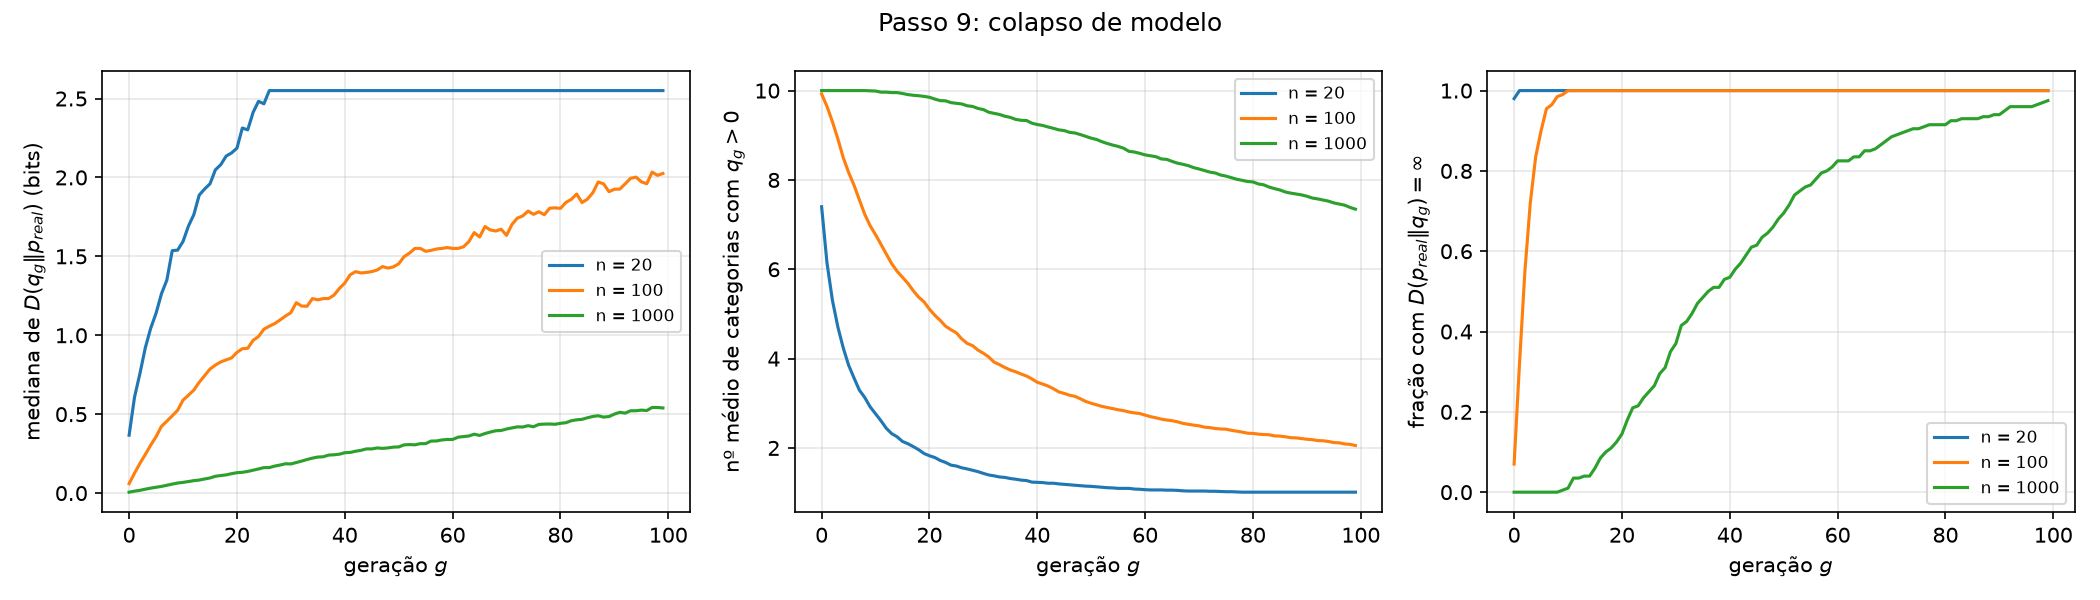
\includegraphics[width=0.95\textwidth]{fig_t2_passo9.png}
  \caption{Evolução do colapso de modelo ao longo de 100 gerações para $n\in\{20, 100, 1000\}$: divergência $D(q_g\|p_{\text{real}})$, número médio de categorias sobreviventes e fração de trajetórias com $D(p_{\text{real}}\|q_g)=\infty$.}
  \label{fig:t2_p9}
\end{figure}

Como mostra a Figura~\ref{fig:t2_p9}, sempre que uma categoria de menor probabilidade deixa de ser sorteada em uma geração, seu peso passa a ser zero em todas as gerações futuras, levando a divergência $D(p_{\text{real}}\|q_g)$ ao infinito. Acompanhando a divergência reversa $D(q_g\|p_{\text{real}})$ e o número de categorias ativas, fica claro o efeito do tamanho amostral: com $n=20$, as caudas desaparecem rapidamente e na geração 50 restam em média apenas $1{,}15$ categorias vivas ($H(q_g)\approx 0{,}11$ bits), colapsando a distribuição em um único estado absorvente. Com $n=1\,000$, o processo é bem mais lento (mantendo $7{,}34$ categorias vivas e $H\approx 2{,}33$ bits na geração 100), mas a perda progressiva de diversidade ocorre de forma inevitável.

%======================================================================
\section{Tópico 3: Compressão de Dados, AEP e Critério de Kelly}

\subsection{Comparação de estratégias e Propriedade de Equipartição Assintótica}
Simulamos uma temporada de apostas esportivas com $m=3$ resultados de probabilidades reais $p=(0{,}5;\,0{,}3;\,0{,}2)$, o que resulta em entropia $H(p)\approx 1{,}485$ bits, e cotações uniformes justas $o_i=3$. Geramos $1\,000$ temporadas independentes de $n=1\,000$ rodadas cada, acompanhando a evolução do patrimônio em escala logarítmica ($\log_2(S_n/S_0) = \sum_{j=1}^n \log_2(b_{X_j}o_{X_j})$) para comparar três estratégias: apostar tudo no favorito ($b=(1,0,0)$), distribuir igualmente ($b_i=1/3$) e apostar segundo o critério de Kelly ($b_i=p_i$).

\begin{figure}[htbp]
  \centering
  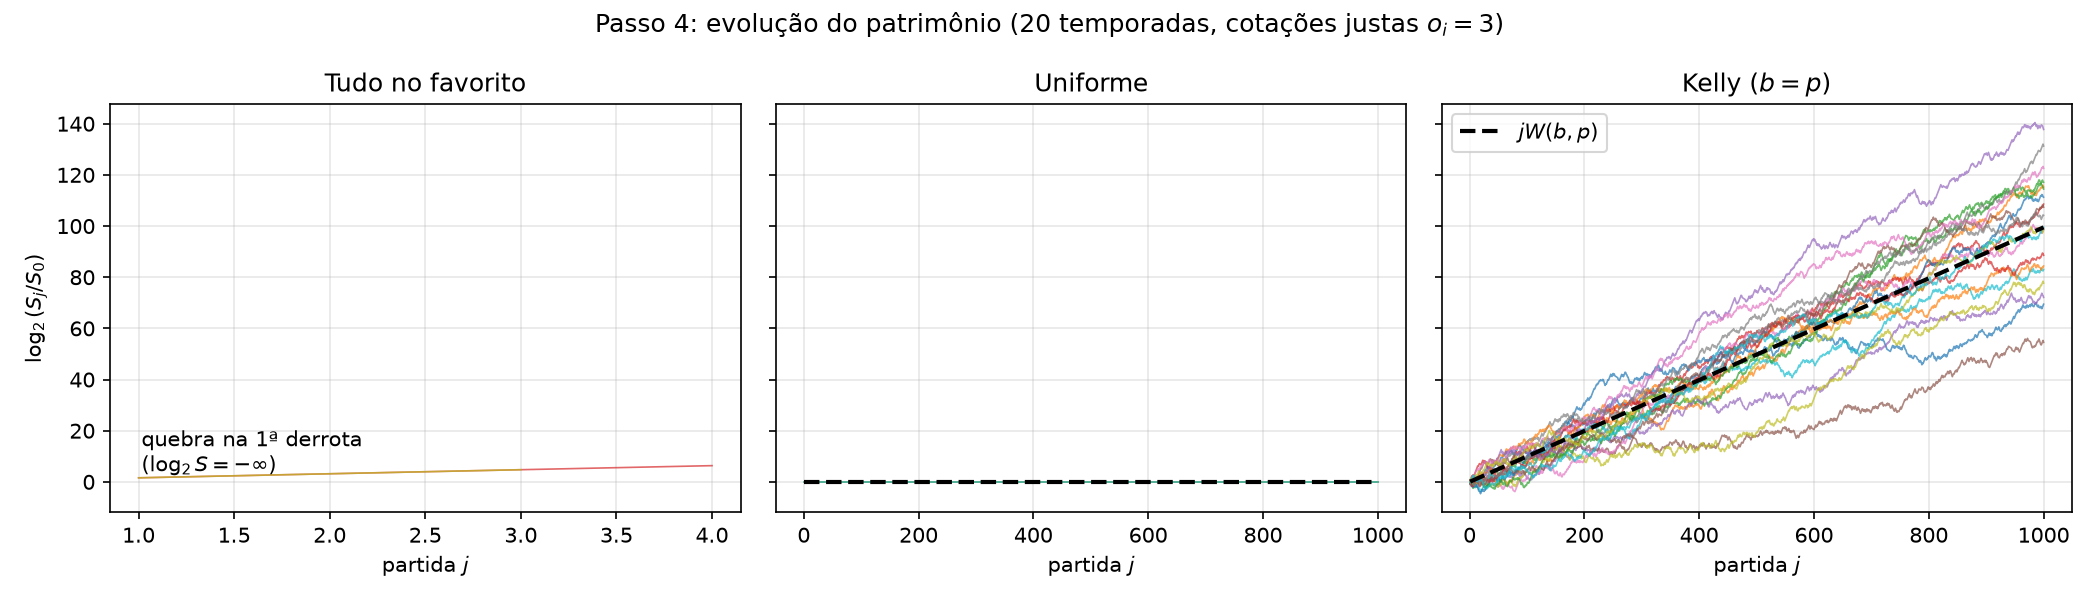
\includegraphics[width=0.92\textwidth]{fig_t3_passo4.png}
  \caption{Evolução do logaritmo do patrimônio $\log_2(S_j/S_0)$ ao longo de uma temporada de 1\,000 partidas.}
  \label{fig:t3_p4}
\end{figure}

\begin{table}[htbp]
  \centering
  \caption{Desempenho das três estratégias em 1\,000 temporadas de $n=1\,000$ apostas ($o_i=3$).}
  \label{tab:t3_p6}
  \resizebox{\textwidth}{!}{\begin{tabular}{lrrrrrr}
\toprule
Estratégia & $W(b,p)$ & Taxa média & Taxa mediana & $S_n<10^{-3}S_0$ & $S_n>10^{3}S_0$ & $\frac1n\log_2 E[S_n]$ \\
\midrule
Tudo no favorito & $-\infty$ & $-\infty$ & $-\infty$ & 100.0\% & 0.0\% & 0.5850 \\
Uniforme & 0.0000 & 0.0000 & 0.0000 & 0.0\% & 0.0\% & 0.0000 \\
Kelly ($b=p$) & 0.0995 & 0.0998 & 0.1001 & 0.0\% & 100.0\% & 0.1890 \\
\bottomrule
\end{tabular}
}
\end{table}

Os resultados na Figura~\ref{fig:t3_p4} e na Tabela~\ref{tab:t3_p6} evidenciam o contraste entre o retorno médio aritmético e a taxa de crescimento típica. Embora apostar tudo no favorito maximize o valor esperado $\frac{1}{n}\log_2 E[S_n] \approx 0{,}585$ bits (dominado pelo evento de probabilidade $0{,}5^{1000}$ em que o favorito vence todas as partidas), na prática o apostador vai à falência na primeira derrota ($100\%$ de ruína nas simulações, $W=-\infty$). A aposta uniforme preserva o capital fixo ($W=0$ pois $b_i o_i = 1$), enquanto a estratégia de Kelly apresenta crescimento exponencial consistente à taxa teórica $W^* = \log_2 3 - H(p) = 0{,}0995$ bits por partida (média empírica de $0{,}0998$ bits, superando $10^3 S_0$ em todas as temporadas simuladas).

\begin{figure}[htbp]
  \centering
  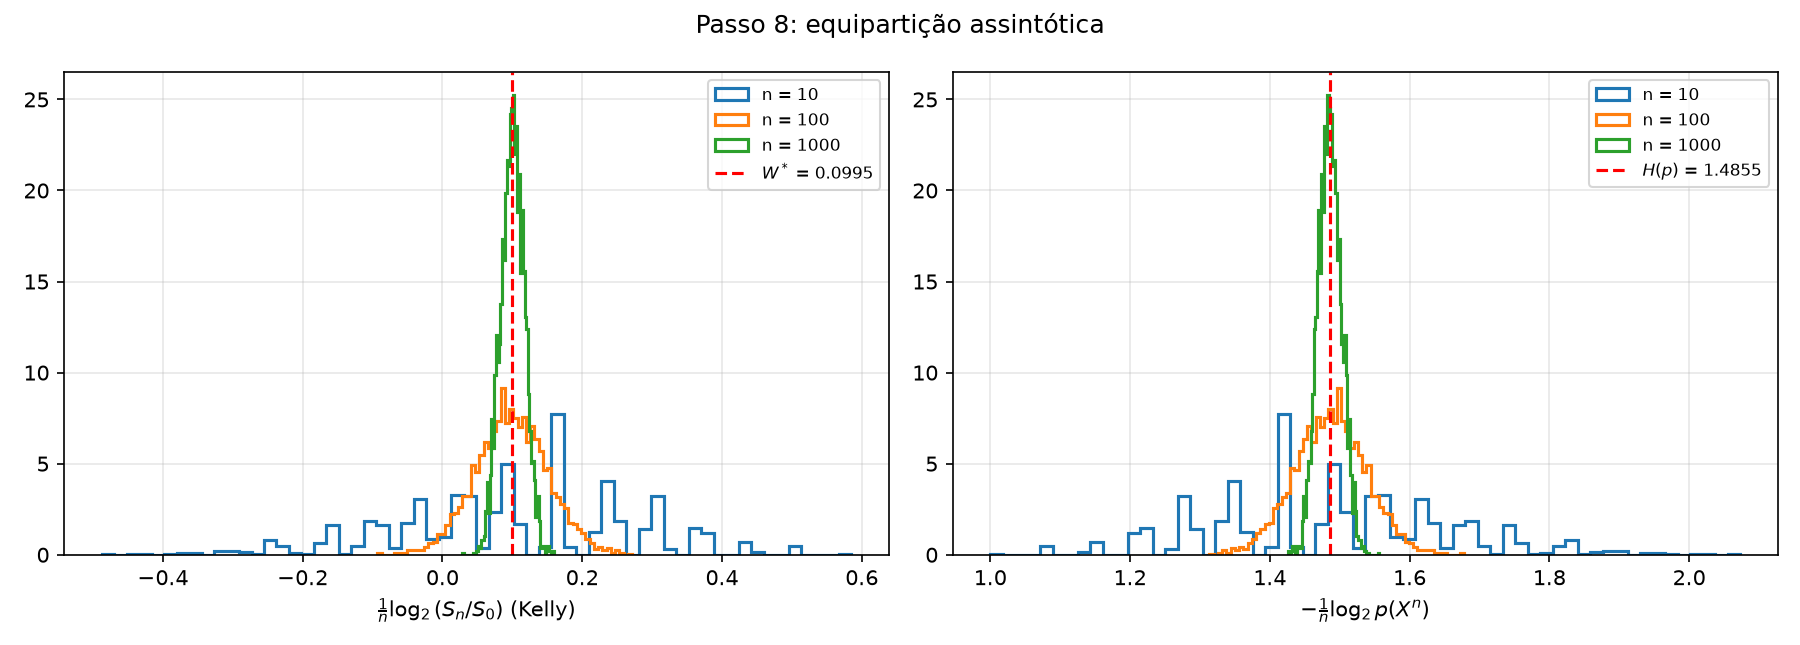
\includegraphics[width=0.92\textwidth]{fig_t3_passo8.png}
  \caption{Concentração da taxa de crescimento de Kelly em torno de $W^*$ (esquerda) e da entropia empírica $-\frac{1}{n}\log_2 p(X^n)$ em torno de $H(p)$ (direita) para $n\in\{10, 100, 1000\}$.}
  \label{fig:t3_p8}
\end{figure}

A conexão direta com a Propriedade de Equipartição Assintótica (AEP) é mostrada na Figura~\ref{fig:t3_p8}. À medida que a duração da temporada aumenta de $n=10$ para $n=1\,000$, a distribuição empírica de $-\frac{1}{n}\log_2 p(X^n)$ concentra-se em torno de $H(p)=1{,}485$ bits e a taxa de Kelly concentra-se em torno de $W^*=0{,}0995$ bits, com desvio padrão caindo na razão $1/\sqrt{n}$ (de $0{,}166$ para $0{,}017$). Com $n=1\,000$, $99{,}7\%$ das sequências geradas pertencem ao conjunto típico com tolerância $\varepsilon=0{,}05$.

\subsection{Informação lateral e custo de crenças incorretas}
Avaliamos em seguida o efeito de uma dica imperfeita $Y$ antes de cada partida, configurada com probabilidade de acerto $P(Y=x\mid X=x)=0{,}60$, o que fornece informação mútua $I(X;Y)=0{,}1981$ bits. Utilizando a estratégia de Kelly condicional $b_i(y)=p(i\mid y)$, a taxa de crescimento média no cenário de cotações justas subiu de $0{,}0995$ para $0{,}2976$ bits, um ganho empírico $\Delta W = 0{,}1977$ bits que concorda com $I(X;Y)$. Repetindo o experimento com cotações de uma casa com margem de lucro, $o=(1{,}8;\,3{,}5;\,5)$, o apostador sem dica tem taxa negativa ($W^*=-0{,}0549$ bits/aposta), mas a informação lateral proporciona exatamente o mesmo acréscimo $\Delta W = 0{,}1977$ bits, tornando a operação lucrativa ($W=+0{,}1432$ bits).

Por outro lado, quando o apostador baseia suas frações de aposta em probabilidades incorretas $q=(0{,}65;\,0{,}20;\,0{,}15)$ (superestimando o favorito), sua taxa de crescimento nas cotações justas cai de $0{,}0995$ para $0{,}0302$ bits por partida. A perda média observada foi de $0{,}0690$ bits, confirmando a previsão teórica $W^* - W(q,p) = D(p\|q) = 0{,}0692$ bits tanto nas cotações justas quanto nas cotações com margem, já que os pagamentos $o_i$ se cancelam na diferença entre os log-retornos das duas estratégias.

%======================================================================
\section{Tópico 4: Capacidade de Canal e Códigos Corretores de Erro}

\subsection{Desempenho dos códigos no canal binário simétrico}
Modelamos o enlace de comunicação espacial como um canal binário simétrico (BSC) com probabilidade de inversão $p=0{,}10$, cuja capacidade teórica é $C = 1 - H_b(0{,}10) \approx 0{,}531$ bits por uso do canal. Comparamos três abordagens de transmissão: envio direto sem codificação ($R=1$), código de repetição com blocos de tamanho ímpar $n_r$ e decisão por maioria ($R=1/n_r$), e o código de Hamming $(7,4)$ ($R=4/7\approx 0{,}571$), implementado via multiplicação matricial em aritmética módulo 2 e decodificação por síndrome ($s = rH^\top \bmod 2$).

\begin{table}[htbp]
  \centering
  \caption{Taxa de transmissão e erro de bit medido e teórico para $p=0{,}10$ ($C\approx 0{,}531$).}
  \label{tab:t4_p7}
  \begin{tabular}{lrrrr}
\toprule
Método & $R$ & Erro de bit (medido) & Erro de bit (teoria) & $R<C$? \\
\midrule
Sem código & 1.000 & 0.1007 & 0.1000 & não \\
Repetição 3x & 0.333 & 0.0278 & 0.0280 & sim \\
Repetição 5x & 0.200 & 0.0087 & 0.0086 & sim \\
Hamming (7,4) & 0.571 & 0.0673 & -- & não \\
Hamming, erro de \emph{bloco} & 0.571 & 0.1495 & 0.1497 & não \\
\bottomrule
\end{tabular}

\end{table}

\begin{figure}[htbp]
  \centering
  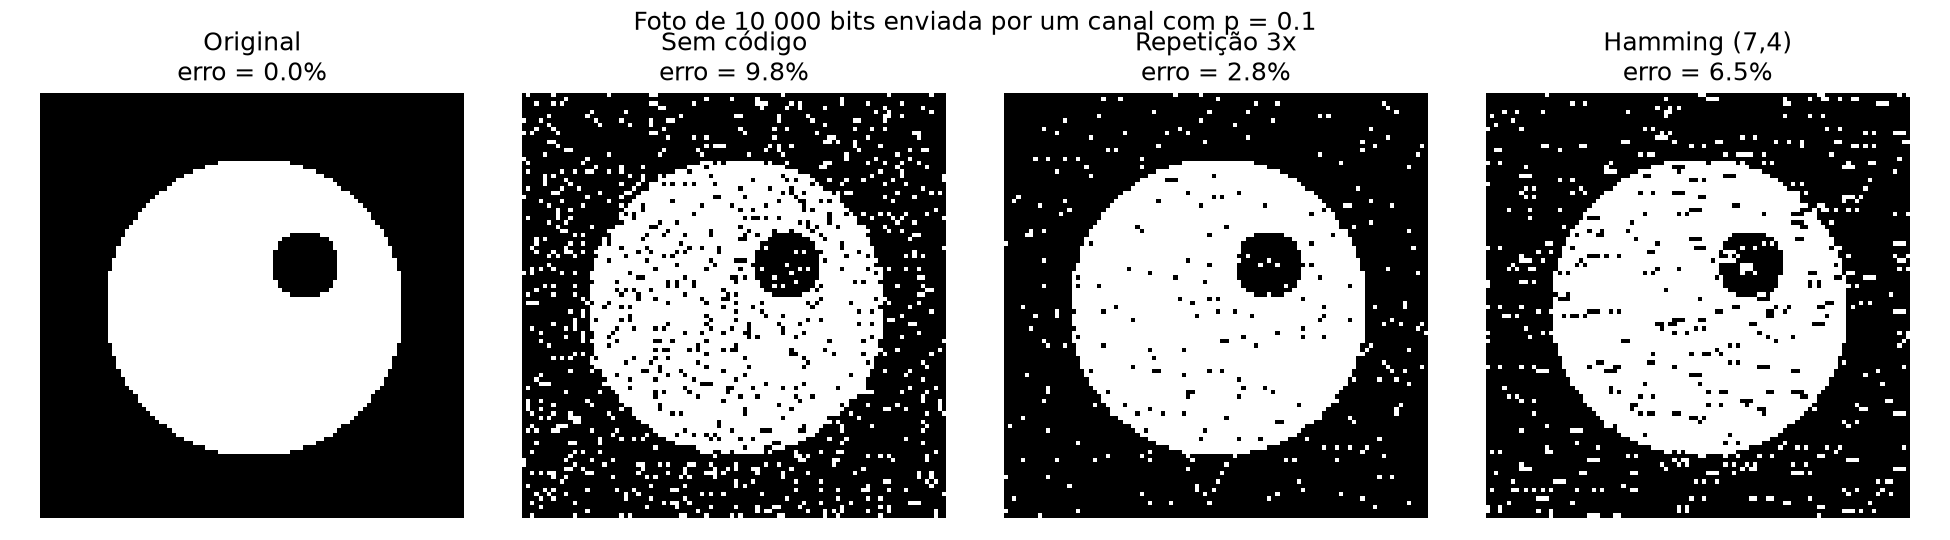
\includegraphics[width=0.92\textwidth]{fig_foto.png}
  \caption{Transmissão de uma imagem binária de $10\,000$ bits pelo canal BSC ($p=0{,}10$) usando os diferentes esquemas de codificação.}
  \label{fig:t4_foto}
\end{figure}

A Tabela~\ref{tab:t4_p7} reúne os resultados numéricos para $p=0{,}10$, e a Figura~\ref{fig:t4_foto} ilustra visualmente a recuperação de uma imagem de $100\times 100$ pixels. A transmissão direta apresenta erro de bit igual ao próprio ruído do canal ($10{,}1\%$). O código de Hamming $(7,4)$ reduz a taxa de erro de bit para $6{,}73\%$, mas como corrige apenas 1 erro por bloco de 7 bits, falha sempre que ocorrem 2 ou mais inversões no mesmo bloco (probabilidade teórica de $14{,}97\%$, medida em $14{,}95\%$), além de operar ligeiramente acima da capacidade ($R=0{,}571 > C$). Já os códigos de repetição $3\times$ ($R=0{,}333$) e $5\times$ ($R=0{,}200$) operam abaixo de $C$ e reduzem a taxa de erro para $2{,}78\%$ e $0{,}87\%$ (concordando com a cauda da distribuição binomial), limpando quase completamente a imagem ao custo de enviar 3 a 5 vezes mais bits pelo canal.

\subsection{Variação do ruído e o limite do Teorema de Shannon}
Na Figura~\ref{fig:t4_p89} (esquerda), variamos a probabilidade de erro do canal $p$ entre $0{,}01$ e $0{,}40$. Para canais pouco ruidosos ($p \le 0{,}05$), tanto o código de Hamming quanto os de repetição derrubam a taxa de erro em várias ordens de grandeza; contudo, conforme $p$ aumenta, a ocorrência de múltiplos erros por bloco torna o Hamming ineficaz antes dos códigos de repetição mais longos.

\begin{figure}[htbp]
  \centering
  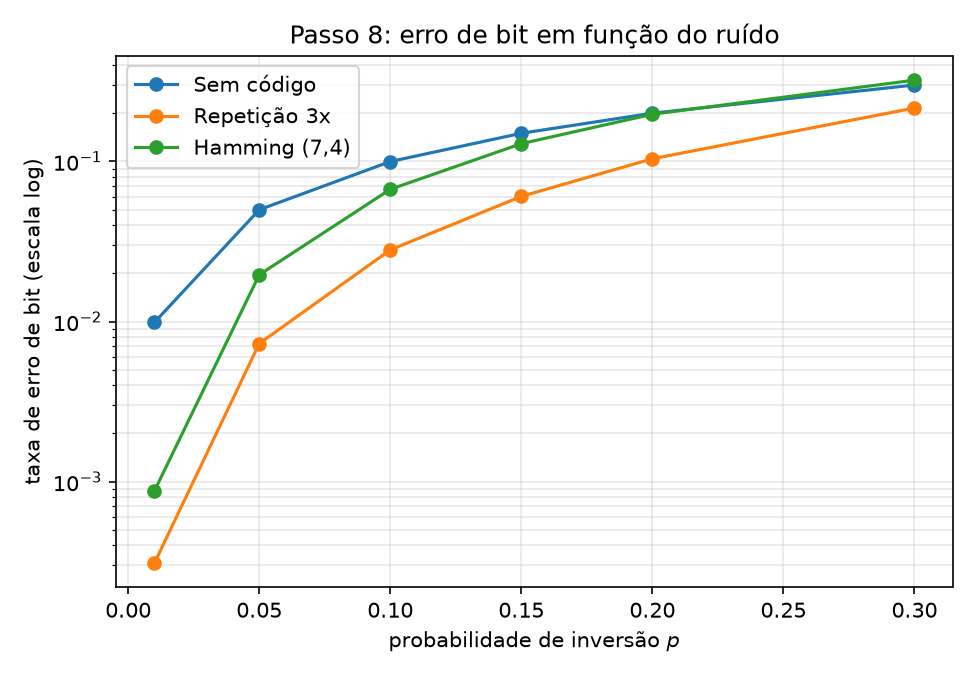
\includegraphics[width=0.48\textwidth]{fig_passo8.png}\hfill
  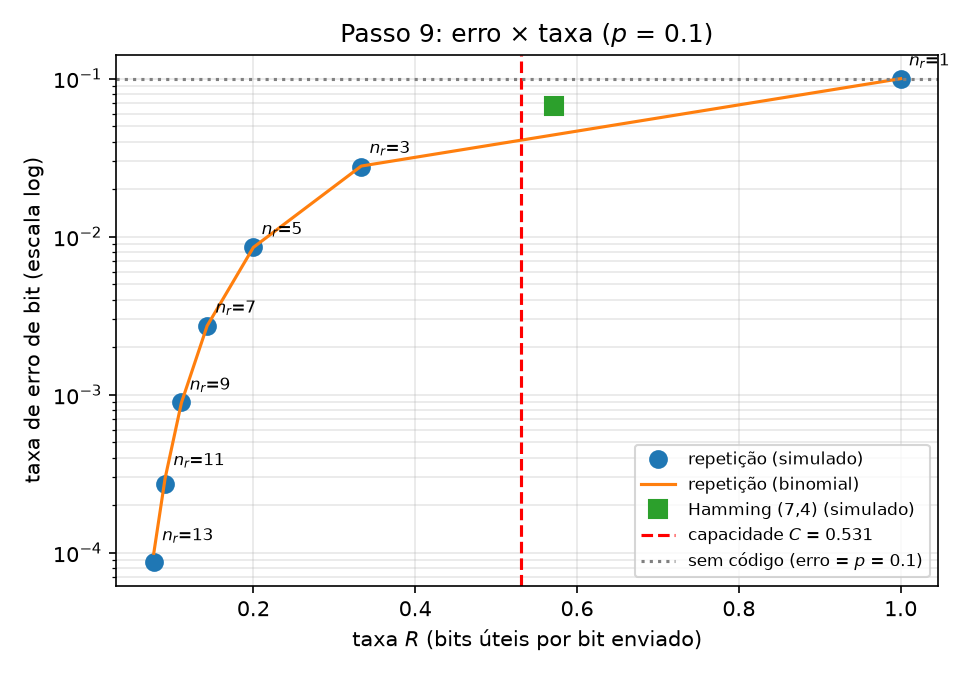
\includegraphics[width=0.48\textwidth]{fig_passo9.png}
  \caption{Esquerda: taxa de erro de bit em função do ruído $p$ do canal. Direita: queda do erro no código de repetição para $n_r$ crescente ($p=0{,}10$), acompanhada da redução da taxa efetiva $R=1/n_r$ em relação à capacidade $C$.}
  \label{fig:t4_p89}
\end{figure}

Na Figura~\ref{fig:t4_p89} (direita), aumentamos o comprimento da repetição de $n_r=1$ até $n_r=13$ fixando $p=0{,}10$. Embora a taxa de erro de bit caia continuamente até $8{,}8\times 10^{-5}$ em $n_r=13$, isso só é alcançado porque a taxa de transmissão $R=1/n_r$ cai para $0{,}077$, afastando-se cada vez mais da capacidade $C\approx 0{,}531$. Esse comportamento contrasta com o Teorema da Codificação de Canal de Shannon, que garante a existência de códigos capazes de atingir probabilidade de erro arbitrariamente pequena mantendo uma taxa $R$ fixa e próxima de $C$, desde que $R<C$ e os blocos codificados sejam suficientemente longos.

Por fim, testamos um cenário mais severo com $p=0{,}20$, onde a capacidade do canal cai para $C\approx 0{,}278$ bits por uso. Nessa condição, todos os esquemas com taxa $R > C$ — sem código ($R=1$), Hamming ($R=0{,}571$) e repetição $3\times$ ($R=0{,}333$) — apresentaram taxas de erro de bit altas ($19{,}9\%$, $19{,}7\%$ e $10{,}4\%$), fazendo com que nenhuma mensagem de 100 bits chegasse intacta ($0{,}0\%$ de sucesso). Somente ao reduzir a taxa para a região $R < C$, usando repetição $5\times$ ($R=0{,}200$, erro de $5{,}8\%$), $9\times$ ($R=0{,}111$, erro de $2{,}0\%$) e $15\times$ ($R=0{,}067$, erro de $0{,}43\%$ e $65{,}1\%$ de mensagens de 100 bits sem erro), foi possível voltar a controlar os erros de transmissão, ilustrando na prática a barreira imposta pela capacidade de Shannon.

\end{document}